\chapter{Introduction}

\section{Graph Theory and Domination}
Graph theory, a branch of discrete mathematics, is the study of graphs. A graph can be considered as a mathematical structure modelling the pairwise relations between various objects. In a graph, the objects are usually represented by nodes while the relation between them is represented by an edge. 
Formally, a graph is an ordered pair $G = (V,E)$ where $V$ denotes the set of vertices, while $E$ denotes the set of edges, each connecting a pair of vertices. An edge $e \in E$ is an ordered pair $e = (u,v)$ which indicates there is a relation between vertices $u \in V$ and $v \in V$. 
\\
A dominating set of a graph $G$ is the subset $D \subseteq V$ such that for any vertex $u \notin D$, there exists a vertex $v \in D$ which is adjacent to $u$. The minimum size of a dominating set $|D|$ of a graph $G$ is called domination number $\gamma(G)$ of the graph.
\\
\begin{figure}[H]
	\centering
	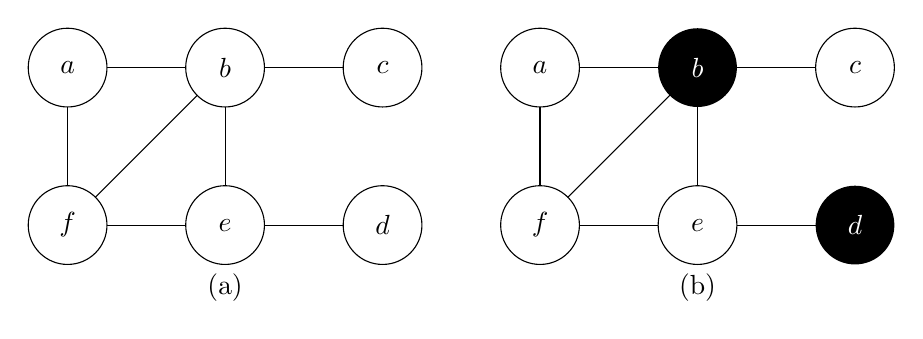
\begin{tikzpicture}
	\draw (0.5,0) -- (1.5,0);
	\draw (2.5,0) -- (3.5,0);
	\draw (0.5,2) -- (1.5,2);
	\draw (2.5,2) -- (3.5,2);
	\draw (0,1.5) -- (0,0.5);
	\draw (0.35,0.35) -- (1.65,1.65);
	\draw (2,1.5) -- (2,0.5);
	
	%\draw (2,2) -- (2,0) -- (0,2);
	
	\draw (0,2) circle(0.5) node{$a$};
	\draw (2,2) circle(0.5) node{$b$};
	\draw (4,2) circle(0.5) node{$c$};
	\draw (4,0) circle(0.5) node{$d$};
	\draw (2,0) circle(0.5) node{$e$};
	\draw (0,0) circle(0.5) node{$f$};
	\draw (2,-0.8) node{(a)};
	
	%-------------------------------------
	\draw (6.5,0) -- (7.5,0);
	\draw (8.5,0) -- (9.5,0);
	\draw (6.5,2) -- (7.5,2);
	\draw (8.5,2) -- (9.5,2);
	\draw (6,1.5) -- (6,0.5);
	\draw (6.35,0.35) -- (7.65,1.65);
	\draw (8,1.5) -- (8,0.5);
	
	%\draw (2,2) -- (2,0) -- (0,2);
	
	\draw (6,2) circle(0.5) node{$a$};
	\fill (8,2) circle(0.5) node[text=white]{$b$};
	\draw (10,2) circle(0.5) node{$c$};
	\fill (10,0) circle(0.5) node[text=white]{$d$};
	\draw (8,0) circle(0.5) node{$e$};
	\draw (6,0) circle(0.5) node{$f$};
	\draw (8,-0.8) node{(b)};
	
	\end{tikzpicture}
	\caption{(a) Graph $G$ (b) Graph $G$ with $\gamma $ set}
\end{figure}
\noindent
In Figure 1.1, the set of vertices $D= \{ b,d\}$ form a minimum dominating set. Note that there can be more than one minimum dominating set for a graph, in Figure 1.3, $\{ b,e \}$ is also a minimum DS. Therefore, $\gamma(G)=2$. \\
\noindent

\section{Historical Background} 
The formal study in graph theory was initiated in 1736, when Leonhard Euler published a paper containing a solution to the famous K{\"{o}}nigsberg bridge problem. He solved the problem by reducing it into graphs, representing lands by vertices and bridges by edges.
\begin{figure}[H]
\centering
\includegraphics[height=6cm,width=10cm]{images/koenisseg.png}
\caption{The K{\"{o}}nigsberg bridge problem}
\end{figure}
The domination problem was first studied around 1862 when de Jaenisch studied the\textit{queen problem}.The queen problem is basically finding the minimum number of queens to place on a $n \times n$ chessboard such that each chess square is covered or dominated by at least one queen.
 \begin{figure}[H]
	\centering
	\includegraphics[height=6cm,width=6cm]{images/Queens.png}
	\caption{The queen problem}
\end{figure}
However, the rigorous study of domination began in 1960s when the term \textit{dominating set} and \textit{domination number} were introduced.

\section{Basic Definition and Terminologies}
\noindent  
Let $G(V,E)$ with $|V|=n$ and $|E(G)|=m$ be a simple, undirected and connected graph. The \textit{open neighborhood} of a vertex $u \in V(G)$ defined as $N_G(u)$= \{$v  | v \in V(G)$ and $(u,v) \in E(G)$\}, similarly the \textit{closed neighborhood} of a vertex $u$ defined as $N_G[u]=N_G(u) \cup \{u\}$. The \textit {degree} of a vertex $u \in V(G)$ is defined as the number of vertices adjacent to $u$ in $G$, hence $d_G(u) = |N_G(u)|$. Specifically, a vertex $u \in V(G)$ is a \textit{pendant vertex} in $G$, if $d_G(u)=1$. The number of pendant vertices in $G$ is denoted by $n_1(G)$. The vertices adjacent to pendant vertex are called a \textit{support vertex}. For a set $S \subseteq V(G)$, let $G[S]$ denote the \textit{subgraph}, \textit{induced by} $S$ in  $G$. Undefined notations and terminology we can refer  \cite{Chartrand,West}.\\
\noindent
A \textit{Dominating Set} (DS) $D$ is a subset of vertices such that  $\forall v \in V(G) \setminus D$, a vertex $u \in D$ exists and $(u,v)\in E(G)$. The \textit{domination number} of $G$ is denoted by $\gamma(G)$ and defined as the minimum cardinality of a dominating set.\\ 

A \textit{Connected Dominating Set} (CDS) $D$ is a subset of vertices such that $D$ is DS of $G$ and $G[D]$ is connected. The \textit{connected domination number} of $G$ is denoted by $\gamma_c(G)$ and defined as the minimum cardinality of a connected dominating set in $G$.\\
\begin{figure}[H]
		\centering
		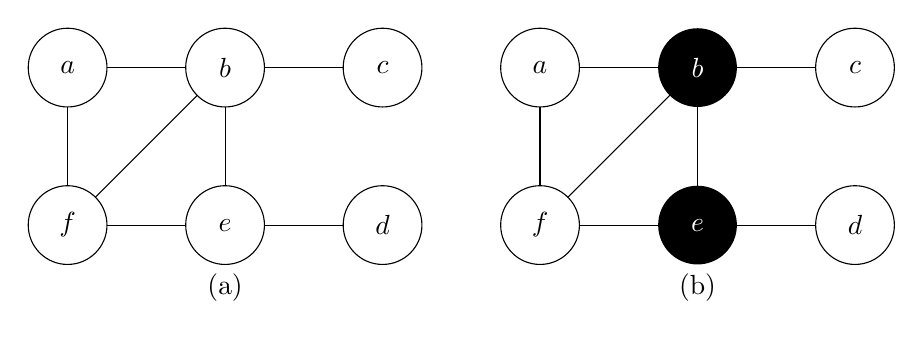
\begin{tikzpicture}
\draw (0.5,0) -- (1.5,0);
\draw (2.5,0) -- (3.5,0);
\draw (0.5,2) -- (1.5,2);
\draw (2.5,2) -- (3.5,2);
\draw (0,1.5) -- (0,0.5);
\draw (0.35,0.35) -- (1.65,1.65);
\draw (2,1.5) -- (2,0.5);

%\draw (2,2) -- (2,0) -- (0,2);

\draw (0,2) circle(0.5) node{$a$};
\draw (2,2) circle(0.5) node{$b$};
\draw (4,2) circle(0.5) node{$c$};
\draw (4,0) circle(0.5) node{$d$};
\draw (2,0) circle(0.5) node{$e$};
\draw (0,0) circle(0.5) node{$f$};
\draw (2,-0.8) node{(a)};

%-------------------------------------
\draw (6.5,0) -- (7.5,0);
\draw (8.5,0) -- (9.5,0);
\draw (6.5,2) -- (7.5,2);
\draw (8.5,2) -- (9.5,2);
\draw (6,1.5) -- (6,0.5);
\draw (6.35,0.35) -- (7.65,1.65);
\draw (8,1.5) -- (8,0.5);

%\draw (2,2) -- (2,0) -- (0,2);

\draw (6,2) circle(0.5) node{$a$};
\fill (8,2) circle(0.5) node[text=white]{$b$};
\draw (10,2) circle(0.5) node{$c$};
\draw (10,0) circle(0.5) node{$d$};
\fill (8,0) circle(0.5) node[text=white]{$e$};
\draw (6,0) circle(0.5) node{$f$};
\draw (8,-0.8) node{(b)};

\end{tikzpicture}
\caption{(a) Graph $G$ (b) Graph $G$ with $\gamma_c$ set}
\end{figure}
\noindent
In Figure 1.4, the set of vertices $D= \{ b,e\}$ form a minimum CDS. Therefore,  $\gamma_c(G)=2$. \\
\noindent
The concept of \textit{doubly connected domination} has been introduced by J. Cyman et al. in \cite{dcds}. A \textit{doubly connected dominating set} (DCDS) $D$ in $G$ is a subset of vertices such that $D$ is a DS of $G$ and $G[V(G)\setminus D]$ and $G[D]$ are connected. The \textit{doubly connected domination number} of $G$ is denoted by $\gamma_{cc}(G)$ and defined as the minimum cardinality of a doubly connected dominating set in $G$.
\begin{figure}[H]
		\centering
		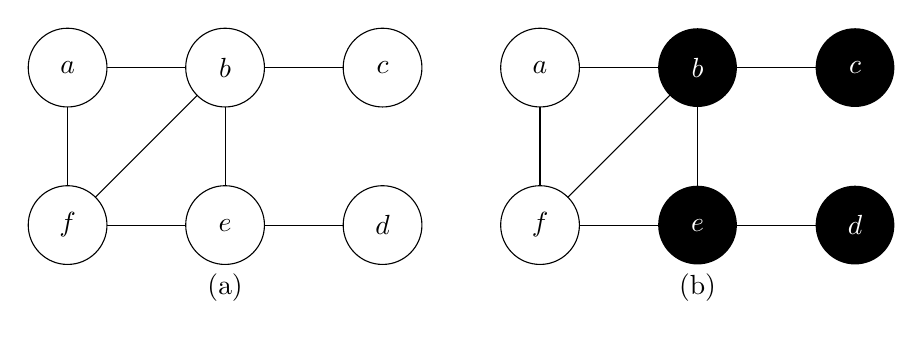
\begin{tikzpicture}
\draw (0.5,0) -- (1.5,0);
\draw (2.5,0) -- (3.5,0);
\draw (0.5,2) -- (1.5,2);
\draw (2.5,2) -- (3.5,2);
\draw (0,1.5) -- (0,0.5);
\draw (0.35,0.35) -- (1.65,1.65);
\draw (2,1.5) -- (2,0.5);

%\draw (2,2) -- (2,0) -- (0,2);

\draw (0,2) circle(0.5) node{$a$};
\draw (2,2) circle(0.5) node{$b$};
\draw (4,2) circle(0.5) node{$c$};
\draw (4,0) circle(0.5) node{$d$};
\draw (2,0) circle(0.5) node{$e$};
\draw (0,0) circle(0.5) node{$f$};
\draw (2,-0.8) node{(a)};

%-------------------------------------
\draw (6.5,0) -- (7.5,0);
\draw (8.5,0) -- (9.5,0);
\draw (6.5,2) -- (7.5,2);
\draw (8.5,2) -- (9.5,2);
\draw (6,1.5) -- (6,0.5);
\draw (6.35,0.35) -- (7.65,1.65);
\draw (8,1.5) -- (8,0.5);

%\draw (2,2) -- (2,0) -- (0,2);

\draw (6,2) circle(0.5) node{$a$};
\fill (8,2) circle(0.5) node[text=white]{$b$};
\fill (10,2) circle(0.5) node[text=white]{$c$};
\fill (10,0) circle(0.5) node[text=white]{$d$};
\fill (8,0) circle(0.5) node[text=white]{$e$};
\draw (6,0) circle(0.5) node{$f$};
\draw (8,-0.8) node{(b)};

\end{tikzpicture}
\caption{(a) Graph $G$ (b) Graph $G$ with $\gamma_{cc}$ set}
\end{figure}
\noindent
In Figure 1.5, the set of vertices $D= \{ b,c,d,e\}$ form a minimum DCDS. Therefore, $\gamma_{cc}(G)=4$. \\
\noindent
E.J. Cockayne et al. has introduced the concept of \textit{secure domination} in \cite{Cockayne}. A \textit{Secure Dominating Set} (SDS) $S$ is a subset of vertices such that for every vertex $v \in V(G) \setminus S$ and a vertex $u \in S$ exists such that there $v$ and $u$ are adjacent and $(S\setminus \{v\}) \cup \{u\}$ is DS of $G$. The \textit{secure domination number}  of $G$ is denoted by $\gamma_s(G)$ and defined as the minimum cardinality of a secure dominating set in $G$.\\
\begin{figure}[H]
		\centering
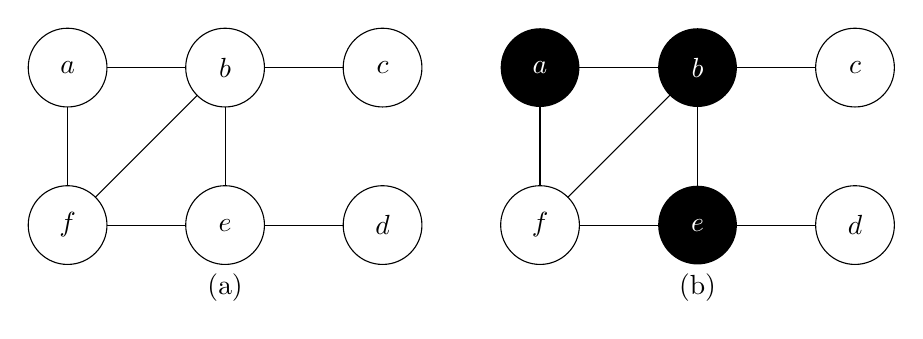
\begin{tikzpicture}
\draw (0.5,0) -- (1.5,0);
\draw (2.5,0) -- (3.5,0);
\draw (0.5,2) -- (1.5,2);
\draw (2.5,2) -- (3.5,2);
\draw (0,1.5) -- (0,0.5);
\draw (0.35,0.35) -- (1.65,1.65);
\draw (2,1.5) -- (2,0.5);

%\draw (2,2) -- (2,0) -- (0,2);

\draw (0,2) circle(0.5) node{$a$};
\draw (2,2) circle(0.5) node{$b$};
\draw (4,2) circle(0.5) node{$c$};
\draw (4,0) circle(0.5) node{$d$};
\draw (2,0) circle(0.5) node{$e$};
\draw (0,0) circle(0.5) node{$f$};
\draw (2,-0.8) node{(a)};

%-------------------------------------
\draw (6.5,0) -- (7.5,0);
\draw (8.5,0) -- (9.5,0);
\draw (6.5,2) -- (7.5,2);
\draw (8.5,2) -- (9.5,2);
\draw (6,1.5) -- (6,0.5);
\draw (6.35,0.35) -- (7.65,1.65);
\draw (8,1.5) -- (8,0.5);

%\draw (2,2) -- (2,0) -- (0,2);


\fill (6,2) circle(0.5) node[text=white]{$a$};
\fill (8,2) circle(0.5) node[text=white]{$b$};
\draw (10,2) circle(0.5) node{$c$};
\draw (10,0) circle(0.5) node{$d$};
\fill (8,0) circle(0.5) node[text=white]{$e$};
\draw (6,0) circle(0.5) node{$f$};

\draw (8,-0.8) node{(b)};
\end{tikzpicture}
\caption{(a) Graph $G$ (b) Graph $G$ with $\gamma_{s}$ set}
\end{figure}
\noindent
In Figure 1.6, the set $S= \{ a,b,e \}$ form a minimum secure dominating set. Therefore, $\gamma_s(G)=3$. \\  
\noindent
The concept of \textit{secure doubly connected domination} has been introduced by B. H. Arriola et al. in \cite{sdcds}. A secure doubly connected dominating set (SDCDS) $S$ in $G$ is a subset of vertices such that $S$ is a DCDS and $\forall v \in S \setminus V(G)$, a vertex $u \in S$ exists where the set $  ( S \setminus \{ u \} ) \cup \{ v \} $ is a DCDS in $G$. The \textit{secure doubly connected domination number} denoted by $\gamma_{scc}(G)$ and defined as the the minimum cardinality of a secure doubly connected dominating set in $G$.
\begin{figure}[H]
		\centering
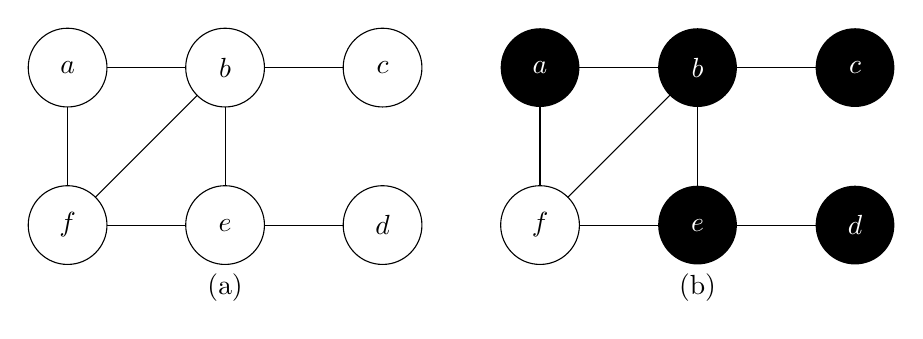
\begin{tikzpicture}
\draw (0.5,0) -- (1.5,0);
\draw (2.5,0) -- (3.5,0);
\draw (0.5,2) -- (1.5,2);
\draw (2.5,2) -- (3.5,2);
\draw (0,1.5) -- (0,0.5);
\draw (0.35,0.35) -- (1.65,1.65);
\draw (2,1.5) -- (2,0.5);

%\draw (2,2) -- (2,0) -- (0,2);

\draw (0,2) circle(0.5) node{$a$};
\draw (2,2) circle(0.5) node{$b$};
\draw (4,2) circle(0.5) node{$c$};
\draw (4,0) circle(0.5) node{$d$};
\draw (2,0) circle(0.5) node{$e$};
\draw (0,0) circle(0.5) node{$f$};
\draw (2,-0.8) node{(a)};

%-------------------------------------
\draw (6.5,0) -- (7.5,0);
\draw (8.5,0) -- (9.5,0);
\draw (6.5,2) -- (7.5,2);
\draw (8.5,2) -- (9.5,2);
\draw (6,1.5) -- (6,0.5);
\draw (6.35,0.35) -- (7.65,1.65);
\draw (8,1.5) -- (8,0.5);

%\draw (2,2) -- (2,0) -- (0,2);

\fill (6,2) circle(0.5) node[text=white]{$a$};
\fill (8,2) circle(0.5) node[text=white]{$b$};
\fill (10,2) circle(0.5) node[text=white]{$c$};
\fill (10,0) circle(0.5) node[text=white]{$d$};
\fill (8,0) circle(0.5) node[text=white]{$e$};
\draw (6,0) circle(0.5) node{$f$};
\draw (8,-0.8) node{(b)};
\end{tikzpicture}
\caption{(a) Graph $G$ (b) Graph $G$ with $\gamma_{scc}$ set}
\end{figure}
\noindent
In Figure 1.7, the set of vertices $S= \{ d,e e,a,b,c \}$ form a minimum secure doubly connected dominating set. Therefore $\gamma_{scc}(G)=5$. \\ 
\noindent
Weichsel has introduced the concept of perfect domination in \cite{Weichsel}. A \textit{Perfect Dominating Set} (PCD) $D$ is a subset of vertices such that  $\forall v \in V(G) \setminus D$, a unique vertex $u \in D$ exists where $u$ and $v$ are adjacent. The \textit{perfect domination number}  of $G$ is denoted by $\gamma_p(G)$ and the minimum cardinality of a perfect dominating set in $G$.\\
\begin{figure}[H]
		\centering
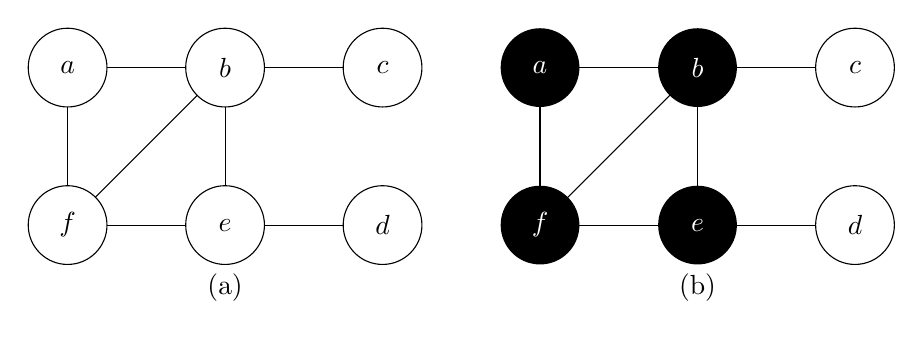
\begin{tikzpicture}
\draw (0.5,0) -- (1.5,0);
\draw (2.5,0) -- (3.5,0);
\draw (0.5,2) -- (1.5,2);
\draw (2.5,2) -- (3.5,2);
\draw (0,1.5) -- (0,0.5);
\draw (0.35,0.35) -- (1.65,1.65);
\draw (2,1.5) -- (2,0.5);

%\draw (2,2) -- (2,0) -- (0,2);

\draw (0,2) circle(0.5) node{$a$};
\draw (2,2) circle(0.5) node{$b$};
\draw (4,2) circle(0.5) node{$c$};
\draw (4,0) circle(0.5) node{$d$};
\draw (2,0) circle(0.5) node{$e$};
\draw (0,0) circle(0.5) node{$f$};
\draw (2,-0.8) node{(a)};

%-------------------------------------
\draw (6.5,0) -- (7.5,0);
\draw (8.5,0) -- (9.5,0);
\draw (6.5,2) -- (7.5,2);
\draw (8.5,2) -- (9.5,2);
\draw (6,1.5) -- (6,0.5);
\draw (6.35,0.35) -- (7.65,1.65);
\draw (8,1.5) -- (8,0.5);

%\draw (2,2) -- (2,0) -- (0,2);

\fill (6,2) circle(0.5) node[text=white]{$a$};
\fill (8,2) circle(0.5) node[text=white]{$b$};
\draw (10,2) circle(0.5) node{$c$};
\draw (10,0) circle(0.5) node{$d$};
\fill (8,0) circle(0.5) node[text=white]{$e$};
\fill (6,0) circle(0.5) node[text=white]{$f$};
\draw (8,-0.8) node{(b)};
\end{tikzpicture}
\caption{(a) Graph $G$ (b) Graph $G$ with $\gamma_p$ set}
\end{figure}
\noindent
In Figure 1.8, the set $D= \{ b,e,f,a \}$ form a minimum perfect dominating set. Therefore, $\gamma_p(G)=4$. \\ 
\noindent
We initiated the study of a variant of secure domination, namely, \textit{secure perfect connected domination}. A { \textit{secure perfect connected dominating set} (SPCDS)} $S$ is a subset of vertices where $G[S]$ is connected and for each vertex $v \in V(G)\setminus S$, a unique vertex $u \in S$ exists such that $u$ and $v$ are adjacent and the set obtained $(S\setminus \lbrace u \rbrace) \cup \lbrace v \rbrace$ is a CDS of $G$. The {\textit{secure perfect connected domination number}} is denoted by {$\gamma_{spc}(G)$} and defined as the minimum cardinality of a SPCDS in $G$.
\begin{figure}[H]
		\centering
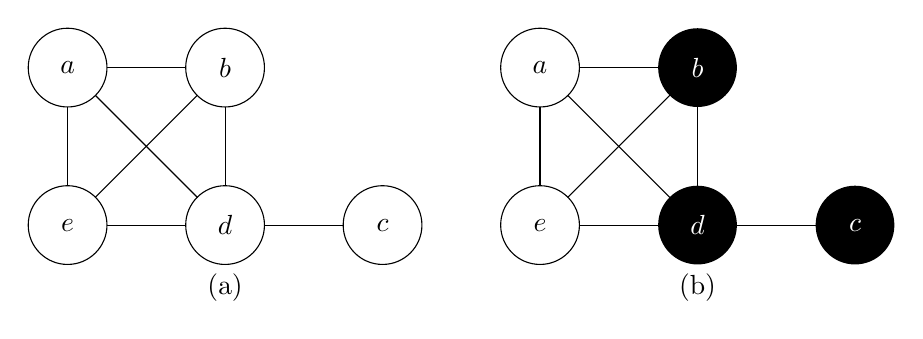
\begin{tikzpicture}
\draw (0.5,0) -- (1.5,0);
\draw (2.5,0) -- (3.5,0);
\draw (0.5,2) -- (1.5,2);
%\draw (2.5,2) -- (3.5,2);
\draw (0,1.5) -- (0,0.5);
\draw (0.35,0.35) -- (1.65,1.65);
\draw (0.35,1.65) -- (1.65,0.35);
\draw (2,1.5) -- (2,0.5);

%\draw (2,2) -- (2,0) -- (0,2);

\draw (0,2) circle(0.5) node{$a$};
\draw (2,2) circle(0.5) node{$b$};
%\draw (4,2) circle(0.5) node{$c$};
\draw (4,0) circle(0.5) node{$c$};
\draw (2,0) circle(0.5) node{$d$};
\draw (0,0) circle(0.5) node{$e$};
\draw (2,-0.8) node{(a)};

%-------------------------------------
\draw (6.5,0) -- (7.5,0);
\draw (8.5,0) -- (9.5,0);
\draw (6.5,2) -- (7.5,2);
%\draw (8.5,2) -- (9.5,2);
\draw (6,1.5) -- (6,0.5);
\draw (6.35,0.35) -- (7.65,1.65);
\draw (6.35,1.65) -- (7.65,0.35);
\draw (8,1.5) -- (8,0.5);

%\draw (2,2) -- (2,0) -- (0,2);

\draw (6,2) circle(0.5) node{$a$};
\fill (8,2) circle(0.5) node[text=white]{$b$};
%\draw (10,2) circle(0.5) node{$c$};
\fill (10,0) circle(0.5) node[text=white]{$c$};
\fill (8,0) circle(0.5) node[text=white]{$d$};
\draw (6,0) circle(0.5) node{$e$};
\draw (8,-0.8) node{(b)};
\end{tikzpicture}
\caption{(a) Graph $G$ (b) Graph $G$ with $\gamma_{spc}$ set}
\end{figure}
\noindent
In Figure 1.9, the set of vertices $S=\{ b,c,d \}$ form a minimum secure perfect connected dominating set. Therefore, $\gamma_{spc}(G)=3$.
\section{Applications of Domination and its Variants}
\subsection{Radio Station}
\noindent
Suppose we need to install a radio station in remote part of the world which has a collection of villages. The radio stations are installed to broadcast the messages to all the villages in the region. Since, radio stations are costly and have limited broadcasting range, we want to install as few radio stations as possible such that messages can be broadcasted to all the villages. We can represent this problem into graph where vertex represents the village and edge represents the distance between two villages. Figure 1.10 shows the representation of village as a graph.
\begin{figure}[H]
\centering
\includegraphics[height=6cm,width=8cm]{images/Village1.png}
    \caption{The collection of villages with distance }
\end{figure}
\noindent
Suppose we are provided the broadcasting range of each radio station then our problem simplifies as to determine the minimum number of radio stations needed such that it dominates all other vertices in graph. First we remove the edges which are more than $50$ km because we have assumed that the broadcasting range of each radio station is not more than $50$ km. Now the problem is reduced to dominating problem and we can easily find the dominating set in the modified graph. Figure 1.11 show the village and its distance only in the range of $50$ km. 
\begin{figure}[H]
\centering
\includegraphics[height=6cm,width=7cm]{images/Village2.png}
    \caption{The collection of villages with distance less than $50$ km}
\end{figure}
\noindent
We can clearly observe that a set $D=\{B, F,H,J\}$ is sufficient to dominate remaining vertices. Thus we can install the radio station at these four places. If we have provided better range of radio station then we may require even less than $4$ radio stations.
\subsection{Bus Routing}
\noindent
In every city many people are traveling by buses. But these buses are having fixed route from one place to other. The organization which manage and decides bus routes, needs to take care that every city must be reachable. Also the nearest bus stop station should be within walkable distance from their current location. There are no bus ride that takes more than some specified number of minutes and limits on the number of passengers that a bus can carry at any one time. Following figure 1.12 represents the street map of a part of city. 
\begin{figure}[H]
\centering
\includegraphics[height=6cm,width=8cm]{images/SchoolBus.png}	
    \caption{Street map of a part of city}
\end{figure}
\noindent
In the above graph edges represents the streets in the city. Now bus organization can decide the bus route such that each passenger can reach to bus stop point by walking at max one block. Thus we can find dominating set such that each block are either a part of bus route or it is a neighbor of the block which are in route. In the above figure the dark line represents the bus route and clearly other vertices not covered in bus route are walkable by at max one block.
\section{Graph Classes}
\subsection{Bipartite Graphs}
\noindent
A graph $G(V_1,V_2,E)$ whose vertex set can be divided into two disjoint independent sets $V_1$ and $V_2$ is called a bipartite graph. A bipartite graph does not have any cycles of odd length. 
\begin{figure}[H]
		\centering
		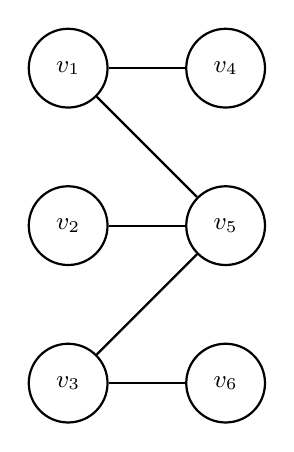
\begin{tikzpicture}[auto, node distance=2.0cm, every loop/.style={}, 
		thick,main node/.style={circle,draw,minimum size=1.0cm,font=\sffamily\small\bfseries}]
			
			\node[main node]  (1) {$v_1$};
			\node[main node] (2) [below of=1] {$v_2$};
			\node[main node] (3) [below of=2] {$v_3$};
			\node[main node] (4) [right of=1] {$v_4$};
			\node[main node] (5) [below of=4] {$v_5$};
			\node[main node] (6) [below of=5]{$v_6$};
			
			
				
			\path[every node/.style={font=\sffamily\small}]
			(1)
			edge node[left] {} (4)
			edge node[left] {} (5)			
									
			(2)
			edge node[left] {} (5)
						
			(3)  
			edge node[left] {} (5)
			edge node[left] {} (6)
			
			;
			\end{tikzpicture}
			\caption{Bipartite graph $G$}
			%\hfill
		\end{figure}
\noindent
Figure 1.13 shows a bipartite graph with $V_1$,$V_2$ being the partite sets. Where $V_1= \{ v_1,v_2,v_3 \}$ and $V_2= \{ v_4,v_5,v_6 \}$. Vertex sets $V_1$ and $V_2$ are independent set.

\subsection{Chordal Graphs}
\noindent
A graph $G(V,E)$ whose all cycles having length four or more in $G$ have a chord is said to be a \textit{chordal graph}. An edge is a chord which is not part of the cycle but connects two vertices of the cycle. 
\begin{figure}[H]
\centering
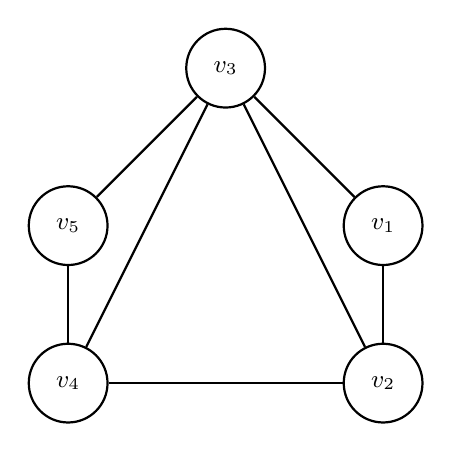
\begin{tikzpicture}[auto, node distance=2.0cm, every loop/.style={},
                    thick,main node/.style={circle,draw,minimum size=1.0cm,font=\sffamily\small\bfseries}]

   \node[main node] (1) {$v_3$};
  \node[main node] (2) [left of=1, below of=1] {$v_5$};
  \node[main node] (3) [right of=1, below of=1] {$v_1$};
  \node[main node] (4) [below of=2] {$v_4$};
  \node[main node] (5) [below of=3] {$v_2$};
  %\node[main node] (6) [below of=5] {};
 


  \path[every node/.style={font=\sffamily\small}]
    (1) %edge node[left] {} (4)
       edge node[left] {} (2)
        edge node[left] {} (3)
        edge node[left] {} (4)
        edge node[left] {} (5)
 
       
    (2) edge node[left] {} (4)
       
       
        
    (3) edge node[left] {}	(5)
    	
    (4)
    	edge node[left] {} (5)
     	
  
     (5)
     
    
       ;
       
\end{tikzpicture}
\caption{Chordal graph $G$}
\end{figure}
\noindent
Figure 1.14 the set $ \{ v_1,v_2,v_4,v_5,v_3\}$ is a cycle and $\{ v_2,v_3\}$, $\{ v_3,v_4\}$ is a chord.


\subsection{Split Graphs}
\noindent
A graph $G(V,E)$ such that whose vertex set $V(G)$ can be partitioned into two disjoint sets $V_1$ and $V_2$ where a clique is formed with vertex set $V_1$ and vertices in $V_2$ form an independent set is said to be a \textit{split graph}. Split graphs is a chordal graphs. \\ \smallskip

\begin{figure}[H]
\centering
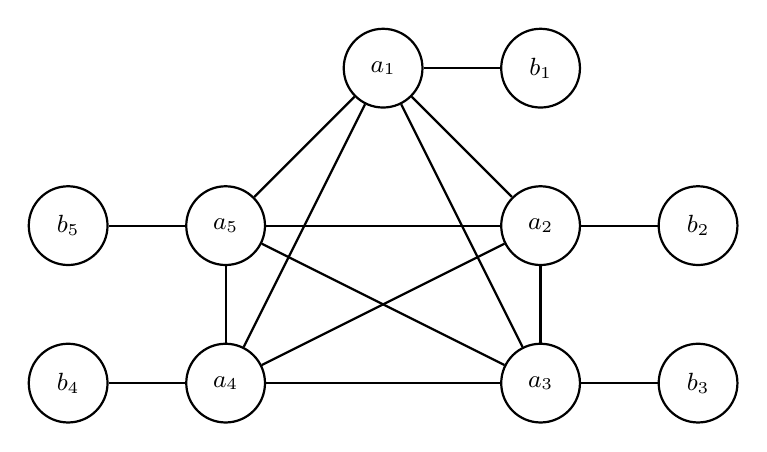
\begin{tikzpicture}[auto, node distance=2.0cm, every loop/.style={},
                    thick,main node/.style={circle,draw,minimum size=1.0cm,font=\sffamily\small\bfseries}]

   \node[main node] (1) {$a_1$};
  \node[main node] (2) [right of=1, below of=1] {$a_2$};
  \node[main node] (3) [below of=2] {$a_3$};
  \node[main node] (5) [left of=1, below of=1] {$a_5$};
  \node[main node] (4) [below of=5] {$a_4$};
  \node[main node] (6) [right of=1] {$b_1$};
  \node[main node] (7) [right of=2] {$b_2$};
  \node[main node] (8) [right of=3] {$b_3$};
  \node[main node] (9) [left of=4] {$b_4$};
  \node[main node] (10) [left of=5] {$b_5$};
 


  \path[every node/.style={font=\sffamily\small}]
    (1) %edge node[left] {} (4)
       edge node[left] {} (2)
        edge node[left] {} (3)
        edge node[left] {} (4)
        edge node[left] {} (5)
        edge node[left] {} (6)
 
       
    (2) edge node[left] {} (3)
    	edge node[left] {} (4)
    	edge node[left] {} (5)
    	edge node[left] {} (7)
       
       
        
    (3) edge node[left] {}	(4)
    	edge node[left] {} (5)
    	edge node[left] {} (8)
    	
    (4)
    	edge node[left] {} (5)
    	edge node[left] {} (9)
     	
  
     (5)
     	edge node[left] {} (10)
    
       ;
       
\end{tikzpicture}
\caption{Split graph $G$}
\end{figure}

\noindent 
Figure 1.15 shows a split graph where $V_1= \{ a_1,a_2,a_3,a_4,a_5 \}$ is a clique and $V_2= \{ b_1,b_2,b_3,b_4,b_5 \}$ is an independent set.

\subsection{Chordal Bipartite Graphs}
\noindent
A bipartite graph $G$ in which every cycle of having length greater than 4 has a chord is a chordal bipartite graph\cite{Brand1}. \\ \smallskip

\begin{figure}[H]
\centering
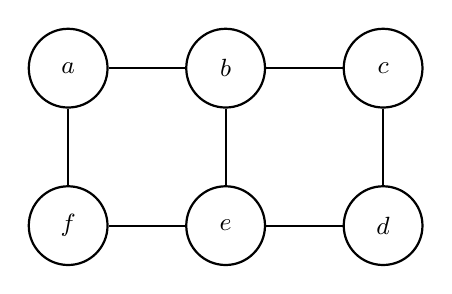
\begin{tikzpicture}[auto, node distance=2.0cm, every loop/.style={},
                    thick,main node/.style={circle,draw,minimum size=1.0cm, font=\sffamily\small\bfseries}]

   \node[main node] (1) {$a$};
  \node[main node] (2) [right of=1] {$b$};
  \node[main node] (3) [right of=2] {$c$};
  \node[main node] (4) [below of=3] {$d$};
  \node[main node] (5) [left of=4] {$e$};
  \node[main node] (6) [left of=5] {$f$};


  \path[every node/.style={font=\sffamily\small}]
    (1) %edge node[left] {} (4)
       edge node[left] {} (2)
        edge node[left] {} (6)
    
       
    (2) edge node[left] {} (3)
    	edge node[left] {} (5)
       
       
        
    (3) edge node[left] {}	(4)
    	
    	
    (4)
    	edge node[left] {} (5)
    	
     	
  
     (5)
     	edge node[left] {} (6)
    
       ;
       
\end{tikzpicture}
\caption{Chordal Bipartite graph $G$}
\end{figure}

\noindent 
Figure 1.16 the set $ \{ a,b,c,d,e,f \}$ is a cycle and $\{ b,c\}$ is a chord.

\subsection{Star Convex Bipartite Graphs}
\noindent
A bipartite graph $G(X,Y,E)$ is a star convex bipartite graph if there is a star $T=(X,F)$ on $X$ such that all vertices of $Y$, its closed neighborhood induces a subtree of $T$ \cite{jiang}. \\ \smallskip

\begin{figure}[H]
		\centering
		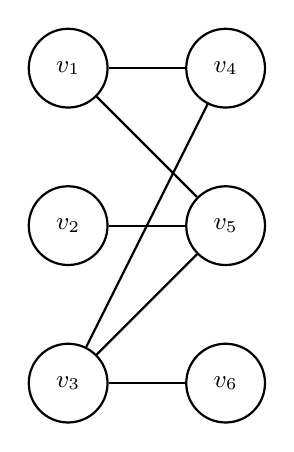
\begin{tikzpicture}[auto, node distance=2.0cm, every loop/.style={}, 
		thick,main node/.style={circle,draw,minimum size=1.0cm,font=\sffamily\small\bfseries}]
			
			\node[main node]  (1) {$v_1$};
			\node[main node] (2) [below of=1] {$v_2$};
			\node[main node] (3) [below of=2] {$v_3$};
			\node[main node] (4) [right of=1] {$v_4$};
			\node[main node] (5) [below of=4] {$v_5$};
			\node[main node] (6) [below of=5]{$v_6$};
			
			
				
			\path[every node/.style={font=\sffamily\small}]
			(1)
			edge node[left] {} (4)
			edge node[left] {} (5)			
									
			(2)
			edge node[left] {} (5)
						
			(3)  
			edge node[left] {} (5)
			edge node[left] {} (6)
			edge node[left] {} (4)			
			
			;
			\end{tikzpicture}
			\caption{Star Convex Bipartite graph $G$}
			%\hfill
		\end{figure}
\noindent
In Figure 1.17, assume tree(star) is formed with vertex set $T= \{ v_1,v_2,v_3\}$ with $v_3$ center vertex then for any vertex from $\{ v_4,v_5, v_6 \}$ its open neighborhood vertex set forms an induce subtree of $T$.

\subsection{Wheel Graphs}
\noindent
A \textit{Wheel graph} denoted by $W_n$ of order $n$ is $K_1 + C_{n-1}$, where $C_{n-1}$ is a cycle of $n-1$ vertices. \\ \smallskip
\begin{figure}[H]
\centering
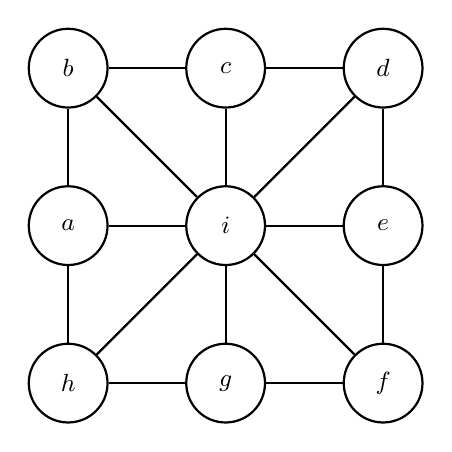
\begin{tikzpicture}[auto, node distance=2.0cm, every loop/.style={},
                    thick,main node/.style={circle,draw,minimum size=1.0cm,font=\sffamily\small\bfseries}]

   \node[main node] (1) {$a$};
   \node[main node] (9) [right of=1]{$i$};
   \node[main node] (5) [right of=9]{$e$};
   \node[main node] (3) [above of=9]{$c$};
   \node[main node] (7) [below of=9]{$g$};
   \node[main node] (2) [above of=1]{$b$};
   \node[main node] (8) [below of=1]{$h$};
   \node[main node] (4) [above of=5]{$d$};
   \node[main node] (6) [below of=5]{$f$};

                        
  


  \path[every node/.style={font=\sffamily\small}]
    (1) %edge node[left] {} (4)
       edge node[left] {} (2)
       
 
       
    (2) edge node[left] {} (3)
    	
       
       
        
    (3) edge node[left] {}	(4)
    	
    (4)
    	edge node[left] {} (5)
    	
     	
  
     (5)
     	edge node[left] {} (6)

     (6)
     	edge node[left] {} (7)
     	(7)
     	edge node[left] {} (8)
     	(8)
     	edge node[left] {} (1)
     (9)
     	edge node[left] {} (1)
     	edge node[left] {} (2)
     	edge node[left] {} (3)
     	edge node[left] {} (4)
     	edge node[left] {} (5)
     	edge node[left] {} (6)
     	edge node[left] {} (7)
     	edge node[left] {} (8)     	

     	    
       ;
       
\end{tikzpicture}
\caption{Wheel graph $W_n$}
\end{figure}

\noindent 
In Figure 1.18, the vertex set $\{ a,b,c,d,e,f,g,h \}$ is a cycle and vertex $\{ i\}$ is common vertex adjacent to all vertices in $W_n$.

\subsection{Fan Graphs}
\noindent
A \textit{Fan graph} $F_n$ is the \textit{join} of $K_1$ with path on $n-1$ vertices i.e. $P_{n-1}$. \\ \smallskip

\begin{figure}[H]
\centering
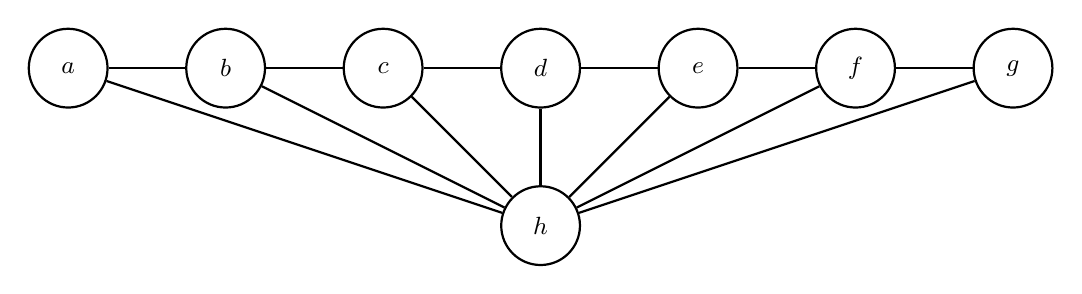
\begin{tikzpicture}[auto, node distance=2.0cm, every loop/.style={},
                    thick,main node/.style={circle,draw,minimum size=1.0cm,font=\sffamily\small\bfseries}]

   \node[main node] (1) {$a$};
   \node[main node] (2) [right of=1]{$b$};
   \node[main node] (3) [right of=2]{$c$};
   \node[main node] (4) [right of=3]{$d$};
   \node[main node] (5) [right of=4]{$e$};
   \node[main node] (6) [right of=5]{$f$};
   \node[main node] (7) [right of=6]{$g$};
   \node[main node] (8) [below of=4]{$h$};
                        
  


  \path[every node/.style={font=\sffamily\small}]
    (1) %edge node[left] {} (4)
       edge node[left] {} (2)
       
 
       
    (2) edge node[left] {} (3)
    	
       
       
        
    (3) edge node[left] {}	(4)
    	
    (4)
    	edge node[left] {} (5)
    	
     	
  
     (5)
     	edge node[left] {} (6)

     (6)
     	edge node[left] {} (7)
     (8)
     	edge node[left] {} (1)
     	edge node[left] {} (2)
     	edge node[left] {} (3)
     	edge node[left] {} (4)
     	edge node[left] {} (5)
     	edge node[left] {} (6)
     	edge node[left] {} (7)

     	    
       ;
       
\end{tikzpicture}
\caption{Fan graph $F_n$}
\end{figure}

\noindent 
In Figure 1.19, the vertex set $\{ a,b,c,d,e,f,g \}$ is a path and vertex $\{ h\}$ is common vertex adjacent to all vertices in $F_n$.

\subsection{Windmill Graphs}
\noindent
The \textit{Windmill graph} denoted by $Wd_{k,n}$ consists of $n$ copies of $K_k$ and identifying one vertex from each $K_k$ copy as a common center vertex. \\ \smallskip

\begin{figure}[H]
\centering
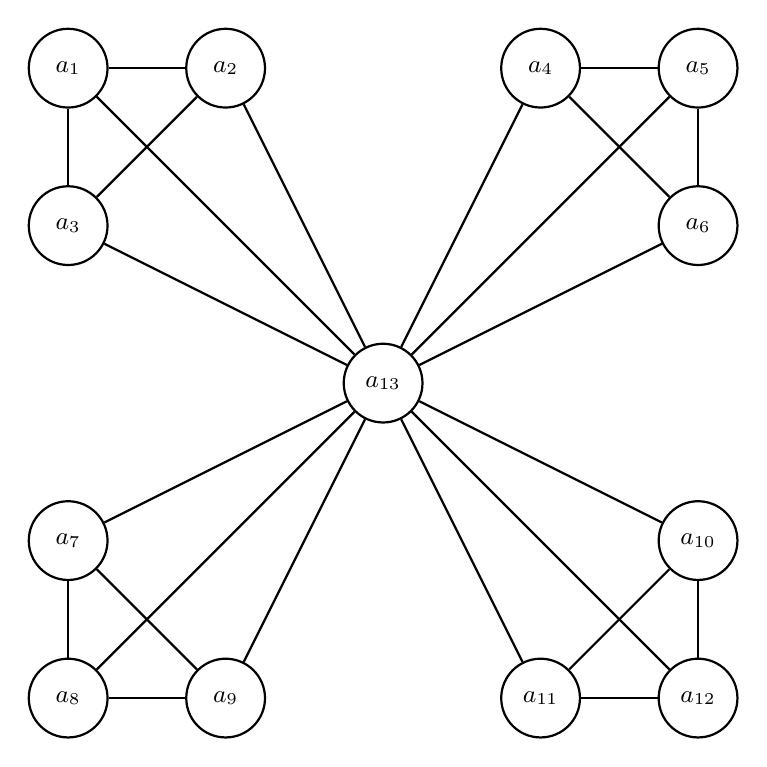
\begin{tikzpicture}[auto, node distance=2.0cm, every loop/.style={},
                    thick,main node/.style={circle,draw,minimum size=1.0cm,font=\sffamily\small\bfseries}]

	\node[main node] (1) {$a_{1}$};
	\node[main node] (2) [right of=1]{$a_{2}$};
	\node (3) [right of=2]{};
	\node[main node] (4) [right of=3]{$a_{4}$};
	\node[main node] (5) [right of=4]{$a_{5}$};
	
	\node[main node] (6) [below of=1]{$a_{3}$};;
	\node (7) [right of=6]{};
	\node (8) [right of=7]{};
	\node (9) [right of=8]{};
	\node[main node] (10) [right of=9]{$a_{6}$};
	
	\node (11) [below of=6]{};
	\node (12) [right of=11]{};
	\node[main node] (13) [right of=12]{$a_{13}$};
	\node (14) [right of=13]{};
	\node (15) [right of=14]{};
	
	\node[main node] (16) [below of=11]{$a_{7}$};;
	\node (17) [right of=16]{};
	\node (18) [right of=17]{};
	\node (19) [right of=18]{};
	\node[main node] (20) [right of=19]{$a_{10}$};
	
	\node[main node] (21) [below of=16]{$a_{8}$};;
	\node[main node] (22) [right of=21]{$a_{9}$};
	\node (23) [right of=22]{};
	\node[main node] (24) [right of=23]{$a_{11}$};
	\node[main node] (25) [right of=24]{$a_{12}$};

  \path[every node/.style={font=\sffamily\small}]
    (1) %edge node[left] {} (4)
       edge node[left] {} (2)
       edge node[left] {} (6)
       
    (2) edge node[left] {} (6)
    	
    (4) edge node[left] {}	(5)
    edge node[left] {}	(10)
    	
    (5)
    	edge node[left] {} (10)
    	
     (16)
     	edge node[left] {} (21)
     	edge node[left] {} (22)

     (21)
     	edge node[left] {} (22)
     	(24)
     	edge node[left] {} (25)
     	edge node[left] {} (20)     	
     	(25)
     	edge node[left] {} (20)
     (13)
     	edge node[left] {} (1)
     	edge node[left] {} (2)
     	edge node[left] {} (4)
     	edge node[left] {} (5)
     	edge node[left] {} (6)
     	edge node[left] {} (10)
     	edge node[left] {} (16)
     	edge node[left] {} (20)
     	edge node[left] {} (21)
     	edge node[left] {} (22)
     	edge node[left] {} (24)
     	edge node[left] {} (25)     	    
       ;
       
\end{tikzpicture}
\caption{Windmill graph $Wd_{k,n}$}
\end{figure}

\noindent 
In Figure 1.20, the vertex sets $\{a_1,a_2,a_3,a_{13}\}$, $\{a_4,a_5,a_6,a_{13}\}$, $\{a_7,a_8,a_9,a_{13}\}$ and $\{a_{10},a_{11},a_{12},a_{13}\}$ are a complete graph $K_4$ and each complete graph shares a common vertex $\{ a_{13}\}$.

\subsection{Trees}
\noindent
A \textit{tree} is an acyclic graph in which there is exactly one path between any two vertices. A tree is always minimally connected, i.e. if an edge is removed from a tree then it becomes a disconnected graph. Let $T(V,E)$ be a tree, where $n$ is the number of vertices, the number of edges is always $n-1$. In a rooted tree, one vertex is designated to be the root. The root has no parent. Non root nodes of degree one are known as leaf nodes, other non root nodes are known as internal nodes.\\
\noindent
Figure 1.21 shows a tree rooted at $v_1$. By $parent(u)$, we denote the parent of vertex $u$. For example, Figure 1.21., $parent(v_2)= v_1$. Similarly, all the children of vertex $v$ are denoted by $children(v)$. For example, in Figure 1.21., $children(v_2)=\{ v_4,v_5 \}$.
\begin{figure}[H]
		\centering
		%\begin{subfigure}%{1\textwidth}
			%\centering
			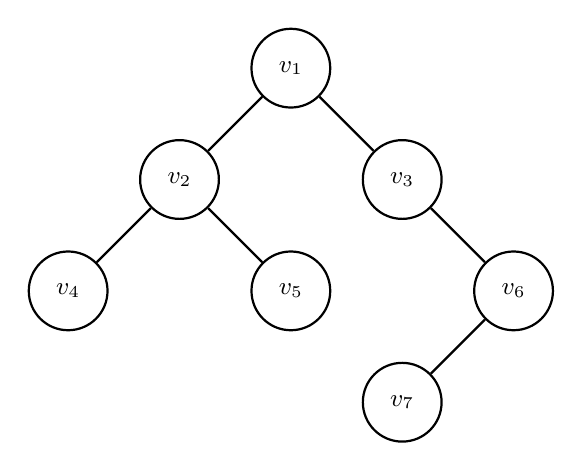
\begin{tikzpicture}[auto, node distance=2.0cm, every loop/.style={},
			thick,main node/.style={circle,draw,minimum size=1.0cm,font=\sffamily\small\bfseries}]
			
			\node[main node] (1) {$v_1$};
			\node[main node] (2) [below left of=1] {$v_2$};
			\node[main node] (3) [below right of=1] {$v_3$};
			\node[main node] (4) [below left of=2] {$v_4$};
			\node[main node] (5) [below right of=2] {$v_5$};
			\node[main node] (6) [below right of=3]{$v_6$};
			\node[main node] (7) [below left of=6]{$v_7$};
			
				
			\path[every node/.style={font=\sffamily\small}]
			(1)
			edge node[left] {} (2)
			edge node[left] {} (3)			
									
			(2)
			edge node[left] {} (4)
			edge node[left] {} (5)
						
			(3)  
			edge node[left] {} (6)
			
			(6)
			edge node[left] {} (7)
			
			;
			\end{tikzpicture}
			\caption{Tree $T$}
			%\hfill
		\end{figure}


\section{Complexity Classes}
\noindent
A complexity class consists of a set of problems for which are solved by an algorithm in $O(f(n))$ exists where $n$ is size of the input. Complexity classes are concerned with the rate of growth of the requirement as the input $n$ increases, the requirement of resources also increases. Complexity classes are defined by bounding either space or time taken by an algorithm. Based on time taken by an algorithm, the complexity classes are categorized into P, NP, NP-hard and NP-complete. 
\subsection{P}
\noindent
A problem belongs to the complexity class P if an algorithm exists, such that it runs for polynomial time on all valid inputs of the problem. Here P stands for polynomial acceptable problems. For the given instance of the problem which belongs to class P, polynomial time is needed to solve the problem. Checking whether a binary tree is  binary search tree or not, finding shortest path in a graph, etc. are examples which belongs to P class.
\subsection{NP}
\noindent
A problem belongs to the complexity class NP if an algorithm exists, such that it runs for non-polynomial time on all valid inputs of the problem. But in polynomial time NP problems can be verified. Here NP stands for non-polynomial acceptable problems. Every NP problem by exhaustive search, it can be solved in exponential time. For every problems in P belong to NP. Whether P=NP or not is still the biggest open question in theoretical computer science, which concerns the relationship between these two classes. The P vs NP problem is one of the seven Millennium Prize Problems chosen by the Clay Mathematical Institute, carrying a prize money of US\$1,000,000 for the one who solves it first. Clique decision problem, independent set problem, dominating set problem, are few examples which belong to NP class.
\subsection{NP-hard}
\noindent
NP-hard problems are at least as hard as NP problems. All NP problems can be reduced to NP-hard in polynomial time. But it is need not to be in NP. Here NP-hard stands for non-deterministic polynomial acceptable problems. The \textit{polynomial time reduction} is a procedure where an instance of a decision problem $Y$ is transformed into an instance of another decision problem $X$ in polynomial time such that if output for the instance of $Y$ is yes, if and only if output for the instance of $X$ is also yes. Thus a problem $X$ is NP-hard if every problem $Y\in NP$ can be polynomially reduced to $X$. Domination problem, secure domination problem, clique decision problem, hamiltonian cycle problem, etc. are few example which belong to NP-hard class.
\subsection{NP-complete}
\noindent
The complexity class NP-complete consists of problems which are both in NP and NP-hard. Here NP-complete stands for non-deterministic polynomial time. The set of NP-complete problems are often denoted by NP-c. NP-complete class consists of the hardest problems in NP. \\
\noindent
Stephen Cook in 1971 and Leonid Levin in 1973 independently proved the first NP-complete problem boolean satisfiability problem (SAT). Since then, thousands of problems have been proved to be NP-complete from various disciplines. A direct consequence which follows that, if SAT can be solved in polynomial time then all the problems in NP can be solved in polynomial time.
\begin{figure}[H]
\centering
\includegraphics[height=5cm,width=7cm]{images/P,NP.png}
    \caption{Euler diagram for the complexity classes when P$\neq$NP and P$=$NP}
\end{figure}
\noindent 
Since a NP-complete problem is both in NP and NP-hard, if we can solve in polynomial time at least one problem which is NP-complete then all other NP problems in polynomial time can be solved, i.e. in such a case P=NP can be proved. In 1971 Richard Karp listed 21 NP-complete problems, a list which consisted of combinatorial and graph theoretic problems \cite{Karp}. Set packing, vertex cover, graph coloring, clique cover, knapsack, are examples of a few example of NP-complete class.
\section{Parameterized Complexity}
\noindent
Many decision problems have a pair of inputs. The domination problem as an example have input $k$ be a positive number and $(G,k)$ as a graph, the problem is to determine minimum DS of a graph $G$ of size at most $k$. Similarly there are many decision problems which takes a pair of inputs.\\
\noindent
Although many of these decision problems are NP-complete. But in practice, these problems requires only small range of inputs. In such cases we can design an algorithm for fixed range of inputs i.e for small range of inputs such that exponential time complexity of an algorithm may become equivalent to polynomial time complexity. This small range of input we call it fixed parameter. For a parameterized problem if an algorithm exists then we call it fixed-parameter tractable. The following are the definition of parameterized problem and fixed-parameter tractable given in \cite{ppc}:
\begin{Definition}
A \textit{parameterized problem} is a set $L \subseteq \Sigma ^* \times \Sigma ^*$ where $ \Sigma $ is a fixed alphabet.
\end{Definition}
\begin{Definition}
A {parameterized problem} $L$ is \textit{fixed-parameter tractable} (FPT) if there exists a constant $\alpha$ and an algorithm to determine if $(x,y)$ is in $L$ in time $f(|y|).|x|^{ \alpha }$, where $f:N \rightarrow N$ is an arbitrary function.
\end{Definition}
\noindent
The vertex cover problem, where for a positive integer $k$ and a given graph $G$, determining a minimum vertex cover set of size at most $k$ of $G$ is NP-complete. If we fixed the input parameter $k$ then there exists an algorithm such that time complexity is $O(2^kn)$ where $n$ is order of graph \cite{ppc} . Hence we can say that vertex cover problem is a FPT. Consider two decision problems $X$ and $Y$. We say that problem $Y$ is polynomial reducible to problem $X$ if for the input of problem $Y$ an algorithm exists such that it is transformed in polynomial time into an input of problem $X$. Therefore we can say that problem $X$ is at least as hard as problem $Y$. Similarly for parameterized problem the definition of parameterized reduction given in \cite{ppc} are as follows:
\begin{Definition}
A reduction of a parameterized problem $L$ to a parameterized problem $L'$ is an oracle  algorithm $A$ that on input $(x,y)$ determines whether $x \in L_y$ and satisfies
\begin{enumerate}[nolistsep]
\item There is an arbitrary function $f:N \rightarrow N$ and a polynomial $q$ such that the  running time of $A$ is bounded by $f(|y|)q(|x|)$.
\item For each $y \in \Sigma^*$ there is a finite subset $J_y \subseteq \Sigma^*$ such that $A$ consults oracles only for fixed-parameter decision problems $L_{w}^{'}$ where $ w \in J_y$.
\end{enumerate}
\end{Definition}
\noindent
Consider the parameterized problem $P$ and $P'$, if $P$ reduces to $P'$ and $P'$ is FPT then $P$ is also FPT. For a parameterized problem if there does not exists any fixed-parameter algorithm then problem is FPT. The hierarchy of parameterized complexity classes given in \cite{ppc} are as follows:
\begin{center}
$FPT \subseteq W[1] \subseteq W[2] \subseteq ... \subseteq W[t]$
\end{center}
\noindent
For a given decision circuit we define \textit{weft} of circuit is the maximum number of large gates on any path from input variable to the output line. A \textit{large gate} is a gate in circuit such that its input variables are more than two. By $P_{f(t,h)}$ we denote a parameterized problem $P$ associated with the family of depth $h$ and  weft $t$ of decision circuit \cite{ppc}. Following are the definition of complexity class W[t]:
\begin{Definition}
A parameterized problem $L$ is to be in W[t] class if and only if $L$ is fixed parameter reducible to the $L_{f(t,h)}$ for some $h$. 
\end{Definition}
\noindent 
Consider an independent set problem, let $k$ be a positive number and a given graph $G$ then it belongs to W[1] class for a fixed parameter $k$ \cite{ppc}. Figure 1.23 shows its equivalent decision circuit, clearly in this circuit there is only one large gate.
\begin{figure}[H]
\centering
\includegraphics[height=5cm,width=7cm]{images/IndependentSet.png}
    \caption{Equivalent decision circuit for independent set}
\end{figure}
\noindent 
Similarly consider domination problem, for a given graph $G$ and $k$ be a positive number then the problem belongs to W[2] class for a fixed parameter $k$  \cite{ppc} . Figure 1.24 shows its equivalent decision circuit, clearly in this circuit there are two large gates.
\begin{figure}[H]
\centering
\includegraphics[height=5cm,width=7cm]{images/DominatingSet.png}
    \caption{Equivalent decision circuit for dominating set}
\end{figure}
\noindent 
\section{Chapter Summary}
\noindent
This thesis is organized in the following manner. \par 
The first chapter begins with a brief introduction of the historical background of graph theory and the concept of domination. The motivation behind studying the concepts of domination, secure domination and its variants has been highlighted with some applications. The concept of secure perfect connected domination which has been introduced in this thesis has been defined. Some special classes of graphs have been discussed and finally the chapter ends with a brief note on the complexity classes. \par
In chapter two, a literature survey of the work on which this dissertation is based upon has been presented. The exact values of $\gamma(G)$, $\gamma_s(G)$, $\gamma_{cc}(G)$ and $\gamma_{scc}(G)$ for some special classes of graphs have been stated. Also a brief summary of the known complexity results of various domination problems have been presented. \par 
In chapter three, the NP-completeness results which have been obtained in our work are presented. We have proved that the doubly connected domination problem is NP-complete for split graphs, chordal bipartite graphs and star convex bipartite graphs. Also we proved that the secure doubly connected domination problem is NP-complete for split graphs and chordal bipartite graphs. \par 
In chapter four, the secure perfect connected domination which we have initiated are defined in our work. We have obtained bounds on secure perfect connected domination number and obtained exact value of secure perfect connected domination number for some classes of graphs in our work are presented.\par
In chapter five, the NP-completeness results which have been obtained in our work are presented. We have proved that the perfect connected domination problem is NP-complete for bipartite graphs. Also we proved that the secure perfect connected domination problem is NP-complete for general graphs. And it is still NP-complete for graphs such as bipartite graphs and star convex bipartite graphs. \par 
In chapter six, the parameterized complexity results which have been obtained in our work are presented. We have proved that the parameterized version of the doubly connected domination is W[2]-hard for split graphs and bipartite graphs. Also we have proved that the parameterized version is W[2]-hard for the secure doubly connected domination problem for split graphs. \par 
In chapter seven, from my work few interesting open problems are listed. 
